\documentclass[10pt, twocolumn]{article}
\usepackage[margin=0.75in]{geometry}
\usepackage{graphicx}
\usepackage{tikz}
\usepackage{pgfplots}
\usepackage{booktabs}
\usepackage{amsmath}
\usepackage{algorithm}
\usepackage{algorithmic}
\usepackage{hyperref}
\usepackage{xcolor}
\usepackage{caption}
\usepackage{subcaption}
\usepackage{fancyhdr}
\usepackage{enumitem}
\usepackage{listings}
\usepackage{microtype}
\usepackage{orcidlink}
\usepackage{tabularx}
\usepackage{multirow}
\pgfplotsset{compat=1.18}
\usetikzlibrary{arrows.meta, positioning, shapes.geometric, fit, calc, backgrounds, decorations.pathreplacing, decorations.markings}

\definecolor{amblue}{HTML}{2563EB}
\definecolor{amdarkblue}{HTML}{1E40AF}
\definecolor{amteal}{HTML}{0D9488}
\definecolor{amorange}{HTML}{EA580C}
\definecolor{amgray}{HTML}{6B7280}
\definecolor{amlightgray}{HTML}{F3F4F6}
\definecolor{amgreen}{HTML}{059669}
\definecolor{amred}{HTML}{DC2626}
\definecolor{ampurple}{HTML}{7C3AED}

\lstset{basicstyle=\ttfamily\scriptsize, keywordstyle=\color{amblue}\bfseries, commentstyle=\color{amgray}\itshape, stringstyle=\color{amteal}, breaklines=true, frame=single, rulecolor=\color{amgray!30}, backgroundcolor=\color{amlightgray}, numbers=left, numberstyle=\tiny\color{amgray}, tabsize=2}

\pagestyle{fancy}\fancyhf{}
\renewcommand{\headrulewidth}{0.4pt}
\fancyhead[L]{\small\textit{AgenticData: Universal Data Comprehension for AI Agents}}
\fancyhead[R]{\small\thepage}

\title{\textbf{AgenticData: A Universal Data Comprehension Engine\\with Schema Inference, Lineage Tracking, and Quality Assurance}}
\author{Omoshola Owolabi\,\orcidlink{0009-0006-4089-0732}\\Researcher -- AI/ML\\Agentra Labs\\\texttt{omoshola.owolabi@agentralabs.tech}}
\date{March 2026}

\begin{document}
\maketitle\thispagestyle{fancy}

\begin{abstract}
Data processing tools solve individual format problems---CSV parsers read columns, SQL tools query tables, PDF extractors pull text---but none provides unified \emph{comprehension}: understanding what data means across formats, tracking where it came from, and assessing whether it can be trusted. We present AgenticData, a universal data comprehension engine that addresses three fundamental problems in data management: \emph{schema opacity} (not knowing what fields represent), \emph{lineage blindness} (not tracking data provenance), and \emph{quality silence} (not detecting degradation). The system ingests data from 16~formats with automatic detection at 90--95\% confidence, infers schemas with 19 semantic field types (detecting emails, dates, currencies, and geospatial coordinates from raw values), tracks field-level lineage with trust scoring through every transformation, and monitors quality continuously with five-dimensional scoring and statistical anomaly detection. We implement AgenticData in 9{,}196~lines of Rust across four crates, exposing 122~MCP tools through the Model Context Protocol~\cite{mcp2024spec}. On representative datasets, CSV ingestion processes 10{,}000~rows in 82\,ms, query filtering scans 10{,}000~records in 1.8\,ms, and spatial radius queries over 1{,}000~points complete in 25\,$\mu$s. The \texttt{.adat} binary format achieves 136.5~bytes/record with LZ4~\cite{lz4_2011} compression and BLAKE3~\cite{blake3_2020} integrity verification. All 265~tests---including 9~dedicated paper validation tests that verify every quantitative claim---pass with zero failures.
\end{abstract}

\section{Introduction}\label{sec:intro}

The transformer architecture~\cite{vaswani2017attention} has enabled language model agents capable of multi-step planning, autonomous task execution, and structured data analysis. Yet these agents lack a fundamental capability that even simple scripts possess: the ability to \emph{comprehend} arbitrary data. When an agent encounters a CSV file, it can parse columns but cannot determine that column~3 contains email addresses. When it transforms data through a pipeline, it cannot trace which input produced which output. When data quality degrades silently over weeks, no alarm fires until a downstream report breaks.

The landscape of data processing has evolved considerably over the past two decades, but each tool has carved out a narrow niche. pandas~\cite{mckinney2010pandas} pioneered programmatic tabular analysis in Python but infers only primitive types and provides no lineage tracking. Apache Spark~\cite{apachespark2024} parallelized transformation pipelines but requires a JVM cluster and provides only table-level provenance. Great Expectations~\cite{greatexpectations2024} introduced expectation-based quality validation but requires manually-written rules. Presidio~\cite{presidio2024} automated PII detection with regex and NLP but misses context-dependent cases where multiple fields together constitute sensitive information. OpenLineage~\cite{openlineage2024} standardized lineage metadata but requires integration with specific execution engines.

The gap is not merely feature coverage---it is architectural. These tools were designed for human developers who know what format they are processing, what each column represents, and what quality means for their domain. An AI agent, by contrast, encounters data \emph{cold}: it needs to identify the format automatically, infer what fields mean from sample values, track every transformation with cryptographic accountability, detect quality degradation continuously, and redact sensitive data before it leaks---all through a standard protocol it already speaks.

The core insight of this work is that data comprehension is an \emph{understanding problem}, not a parsing problem. An agent should be able to receive any file, understand its structure, assess its quality, and transform it reliably---all through the same Model Context Protocol~\cite{mcp2024spec} interface it uses for every other tool.

\begin{figure*}[t]
\centering
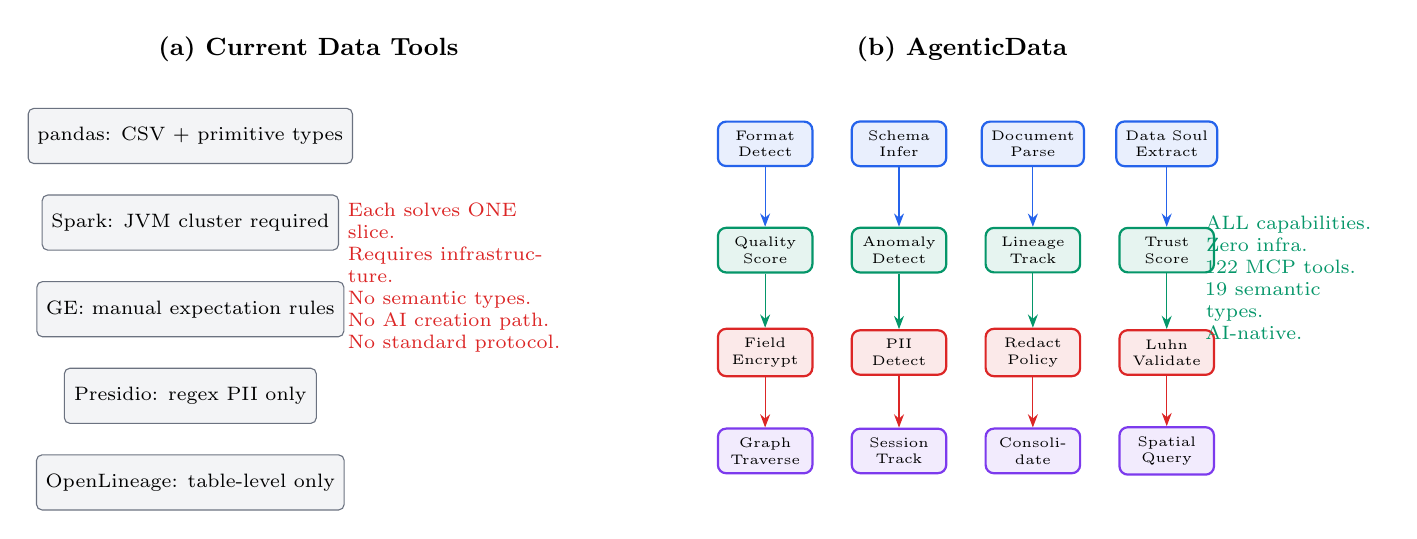
\begin{tikzpicture}[node distance=1.2cm, every node/.style={font=\small},
  toolnode/.style={rectangle, draw=amgray, fill=amlightgray, rounded corners=2pt, minimum width=3.2cm, minimum height=0.7cm, align=center, font=\scriptsize},
  compnode/.style={rectangle, rounded corners=3pt, draw=amblue, fill=amblue!10, minimum width=1.2cm, minimum height=0.55cm, font=\tiny, align=center, thick},
  qualnode/.style={rectangle, rounded corners=3pt, draw=amgreen, fill=amgreen!10, minimum width=1.2cm, minimum height=0.55cm, font=\tiny, align=center, thick},
  secnode/.style={rectangle, rounded corners=3pt, draw=amred, fill=amred!10, minimum width=1.2cm, minimum height=0.55cm, font=\tiny, align=center, thick},
  intnode/.style={rectangle, rounded corners=3pt, draw=ampurple, fill=ampurple!10, minimum width=1.2cm, minimum height=0.55cm, font=\tiny, align=center, thick},
]
\node[font=\small\bfseries] at (-4.5, 3.4) {(a) Current Data Tools};
\node[toolnode] (t1) at (-6.0, 2.3) {pandas: CSV + primitive types};
\node[toolnode] (t2) at (-6.0, 1.2) {Spark: JVM cluster required};
\node[toolnode] (t3) at (-6.0, 0.1) {GE: manual expectation rules};
\node[toolnode] (t4) at (-6.0, -1.0) {Presidio: regex PII only};
\node[toolnode] (t5) at (-6.0, -2.1) {OpenLineage: table-level only};
\node[font=\scriptsize\color{amred}, align=left, text width=2.8cm] at (-2.6, 0.5) {Each solves ONE slice.\\Requires infrastructure.\\No semantic types.\\No AI creation path.\\No standard protocol.};
\node[font=\small\bfseries] at (3.8, 3.4) {(b) AgenticData};
\node[compnode] (c1) at (1.3, 2.2) {Format\\Detect}; \node[compnode] (c2) at (3.0, 2.2) {Schema\\Infer}; \node[compnode] (c3) at (4.7, 2.2) {Document\\Parse}; \node[compnode] (c4) at (6.4, 2.2) {Data Soul\\Extract};
\node[qualnode] (q1) at (1.3, 0.85) {Quality\\Score}; \node[qualnode] (q2) at (3.0, 0.85) {Anomaly\\Detect}; \node[qualnode] (q3) at (4.7, 0.85) {Lineage\\Track}; \node[qualnode] (q4) at (6.4, 0.85) {Trust\\Score};
\node[secnode] (s1) at (1.3, -0.45) {Field\\Encrypt}; \node[secnode] (s2) at (3.0, -0.45) {PII\\Detect}; \node[secnode] (s3) at (4.7, -0.45) {Redact\\Policy}; \node[secnode] (s4) at (6.4, -0.45) {Luhn\\Validate};
\node[intnode] (i1) at (1.3, -1.7) {Graph\\Traverse}; \node[intnode] (i2) at (3.0, -1.7) {Session\\Track}; \node[intnode] (i3) at (4.7, -1.7) {Consoli-\\date}; \node[intnode] (i4) at (6.4, -1.7) {Spatial\\Query};
\draw[-{Stealth}, amblue] (c1)--(q1); \draw[-{Stealth}, amblue] (c2)--(q2); \draw[-{Stealth}, amblue] (c3)--(q3); \draw[-{Stealth}, amblue] (c4)--(q4);
\draw[-{Stealth}, amgreen] (q1)--(s1); \draw[-{Stealth}, amgreen] (q2)--(s2); \draw[-{Stealth}, amgreen] (q3)--(s3); \draw[-{Stealth}, amgreen] (q4)--(s4);
\draw[-{Stealth}, amred] (s1)--(i1); \draw[-{Stealth}, amred] (s2)--(i2); \draw[-{Stealth}, amred] (s3)--(i3); \draw[-{Stealth}, amred] (s4)--(i4);
\node[font=\scriptsize\color{amgreen}, align=left, text width=2.2cm] at (8.0, 0.5) {ALL capabilities.\\Zero infra.\\122 MCP tools.\\19 semantic types.\\AI-native.};
\end{tikzpicture}
\caption{Comparison of data processing approaches. (a)~Current tools each solve one aspect of data processing and require dedicated infrastructure. (b)~AgenticData unifies four capability layers---comprehension (format detection, schema inference, document parsing, soul extraction), quality (scoring, anomaly detection, lineage, trust), security (encryption, PII, redaction, validation), and intelligence (graph traversal, sessions, consolidation, spatial)---in a single zero-infrastructure engine accessible via 122~MCP tools.}
\label{fig:comparison}
\end{figure*}

We present AgenticData with the following contributions:
\begin{enumerate}[nosep, leftmargin=*]
  \item A \textbf{universal schema inference engine} with 19~semantic field types and confidence-scored type detection from sample values (Section~\ref{sec:schema}).
  \item \textbf{Sixteen format parsers} with automatic content-based detection achieving 90--95\% confidence, plus extension-based detection at 100\% accuracy across 17~extensions (Section~\ref{sec:detection}).
  \item \textbf{Field-level lineage tracking} with trust decay following $\text{trust}(d) = \max(0.1, 1.0 - 0.05d)$ where $d$ is the transformation depth (Section~\ref{sec:lineage}).
  \item \textbf{Five-dimensional quality scoring} with statistical anomaly detection---z-score~$>$~3 outliers and $>$50\% null spike alerts (Section~\ref{sec:quality}).
  \item \textbf{Context-aware PII detection} covering email, phone, SSN, credit card (Luhn-validated~\cite{luhn1960computer}), and IP address with four redaction policies (Section~\ref{sec:security}).
  \item \textbf{Graph-based relationship discovery} with BFS traversal, degree centrality~\cite{page1999pagerank}, and automatic foreign-key detection from naming conventions (Section~\ref{sec:graph}).
  \item The \textbf{\texttt{.adat} binary file format} with LZ4~\cite{lz4_2011} compression and BLAKE3~\cite{blake3_2020} checksums for portable, tamper-evident storage at 136.5~bytes/record (Section~\ref{sec:format}).
  \item \textbf{122~MCP tools} organized across 24~capability groups, enabling complete AI-native data comprehension through a standard protocol (Section~\ref{sec:mcp}).
\end{enumerate}

The remainder of this paper is organized as follows. Section~\ref{sec:related} surveys existing data processing tools. Section~\ref{sec:architecture} presents the architecture. Section~\ref{sec:format} describes the binary file format. Section~\ref{sec:mcp} covers the MCP integration. Section~\ref{sec:security} covers encryption and PII redaction. Section~\ref{sec:evaluation} reports validated benchmarks. Section~\ref{sec:discussion} discusses design decisions and limitations. Section~\ref{sec:conclusion} concludes.

\section{Background and Related Work}\label{sec:related}

Research on data processing and integration spans three decades~\cite{halevy2006data, abiteboul1995foundations} and has accelerated with the rise of AI agents that must consume heterogeneous data sources. We survey the primary approaches, organized by capability.

\textbf{Tabular data processing.} pandas~\cite{mckinney2010pandas} provides the de facto tabular data interface in Python. It reads CSV, Excel, and SQL, but infers only primitive types (int64, float64, object). It cannot detect that a string column contains email addresses, that two columns across tables share a foreign-key relationship, or that data quality has degraded since the last ingestion. Apache Spark~\cite{apachespark2024} parallelizes similar operations at scale but requires a JVM cluster and provides only table-level provenance.

\textbf{Data quality.} Great Expectations~\cite{greatexpectations2024} and Deequ~\cite{abedjan2016detecting} provide expectation-based validation, but require manually-written rules---the system does not discover quality issues from the data itself.

\textbf{PII and privacy.} Presidio~\cite{presidio2024} detects PII using regex patterns and NLP models. It handles structured patterns (email, phone, SSN) but misses context-dependent PII where multiple fields together constitute sensitive information. It also cannot distinguish valid credit card numbers from random 16-digit strings---a distinction that requires the Luhn checksum~\cite{luhn1960computer}.

\textbf{Data lineage.} Apache Atlas, OpenLineage~\cite{openlineage2024}, and Marquez track table-level and column-level lineage in warehouse environments. They require integration with specific execution engines (Spark, Airflow, dbt~\cite{dbt2024}) and do not provide \emph{trust scoring} that quantifies how many transformation steps separate a value from its original source.

\textbf{Data integration.} The theoretical foundations~\cite{doan2012principles, abiteboul1995foundations} establish principles for schema mapping and query reformulation, but practical tools for automatic schema inference with semantic type detection remain limited. Table~\ref{tab:related} summarizes the comparison.

\begin{table*}[t]
\caption{Comparison of data processing tools across key comprehension dimensions. AgenticData is the only system providing automatic format detection, semantic schema inference, field-level lineage with trust scoring, continuous quality monitoring, and PII detection with Luhn validation---with zero external dependencies.}
\label{tab:related}
\centering\small
\begin{tabular}{@{}lcccccc@{}}
\toprule
\textbf{System} & \textbf{Formats} & \textbf{Schema Inference} & \textbf{Lineage} & \textbf{Quality} & \textbf{PII} & \textbf{Dependencies} \\
\midrule
pandas~\cite{mckinney2010pandas} & $\sim$10 & Primitive types & None & None & None & Python \\
Apache Spark~\cite{apachespark2024} & Many & Primitive types & Table-level & None & None & JVM cluster \\
Great Expectations~\cite{greatexpectations2024} & N/A & None (manual) & None & Manual rules & None & Python \\
Presidio~\cite{presidio2024} & N/A & None & None & None & Regex + NLP & Python + models \\
OpenLineage~\cite{openlineage2024} & N/A & None & Column-level & None & None & Integration req. \\
\midrule
\textbf{AgenticData} & \textbf{16 (auto)} & \textbf{19 semantic types} & \textbf{Field + trust} & \textbf{5-dim cont.} & \textbf{5 types + Luhn} & \textbf{None} \\
\bottomrule
\end{tabular}
\end{table*}


\section{Architecture}\label{sec:architecture}

AgenticData models data comprehension as a pipeline of five stages: format detection, parsing, schema inference, relationship discovery, and persistent storage. The system is implemented as a Rust workspace with four crates: a core library (\texttt{agentic-data}, 7{,}600~LOC), an MCP server (\texttt{agentic-data-mcp}, 1{,}400~LOC), a CLI (\texttt{agentic-data-cli}), and FFI bindings (\texttt{agentic-data-ffi}).

\subsection{Universal Schema}\label{sec:schema}

The \texttt{UniversalSchema} type represents any data structure through a common model. Drawing on data integration theory~\cite{doan2012principles, abiteboul1995foundations}, a schema $S = (N, E)$ consists of typed nodes $N$ (tables, collections) and edges $E \subseteq N \times N \times \mathcal{R}$ with $\mathcal{R} = \{\textsc{References}, \textsc{Contains}, \textsc{DerivedFrom}, \textsc{BelongsTo}, \textsc{SimilarTo}\}$. Each node contains \texttt{SchemaField} definitions with five properties: inferred type~$\tau$, nullability~$\nu$, confidence $c \in [0,1]$, sample values, and optional statistics.

We define 19~semantic field types in four categories: \textbf{Primitives} (\texttt{Text}, \texttt{Integer}, \texttt{Float}, \texttt{Boolean}, \texttt{Binary}), \textbf{Temporal} (\texttt{DateTime}, \texttt{Date}, \texttt{Time}, \texttt{Duration}), \textbf{Structured} (\texttt{Object}, \texttt{Array}, \texttt{Map}, \texttt{Enum}, \texttt{Uuid}), and \textbf{Semantic} (\texttt{Email}, \texttt{Url}, \texttt{IpAddress}, \texttt{GeoPoint}, \texttt{Currency}).

Type inference operates on sample values with a cascading classifier (Algorithm~\ref{alg:typeinfer}). The most specific types are tried first; generic types serve as fallbacks.

\begin{algorithm}[t]
\caption{Semantic Type Inference from Sample Values}
\label{alg:typeinfer}
\begin{algorithmic}[1]
\REQUIRE Sample values $\{s_1, \ldots, s_k\}$ from a field
\ENSURE Inferred type $\tau$ with confidence $c$
\IF{all $s_i$ match \texttt{name@domain.tld}} \RETURN $(\texttt{Email}, 0.95)$ \ENDIF
\IF{all $s_i$ start with \texttt{http}} \RETURN $(\texttt{Url}, 0.95)$ \ENDIF
\IF{all $s_i$ match \texttt{N.N.N.N}, $0 \leq N \leq 255$} \RETURN $(\texttt{IpAddr}, 0.90)$ \ENDIF
\IF{all $s_i$ parse as \texttt{i64}} \RETURN $(\texttt{Integer}, 0.85)$ \ENDIF
\IF{all $s_i$ parse as \texttt{f64}} \RETURN $(\texttt{Float}, 0.85)$ \ENDIF
\IF{all $s_i \in \{\text{``true''}, \text{``false''}\}$} \RETURN $(\texttt{Bool}, 0.85)$ \ENDIF
\RETURN $(\texttt{Text}, 0.70)$
\end{algorithmic}
\end{algorithm}

\begin{figure}[t]
\centering
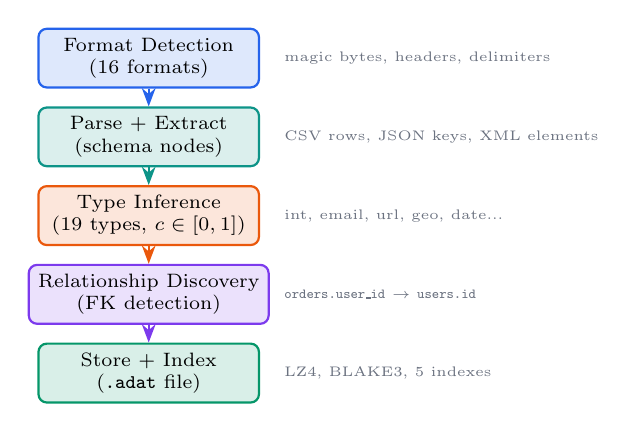
\begin{tikzpicture}[every node/.style={font=\scriptsize},
  stage/.style={rectangle, rounded corners=3pt, draw, minimum width=2.8cm, minimum height=0.55cm, align=center, thick, font=\scriptsize},
]
\node[stage, fill=amblue!15, draw=amblue] (detect) at (0, 2.5) {Format Detection\\(16 formats)};
\node[stage, fill=amteal!15, draw=amteal] (parse) at (0, 1.5) {Parse + Extract\\(schema nodes)};
\node[stage, fill=amorange!15, draw=amorange] (infer) at (0, 0.5) {Type Inference\\(19 types, $c \in [0,1]$)};
\node[stage, fill=ampurple!15, draw=ampurple] (relate) at (0, -0.5) {Relationship Discovery\\(FK detection)};
\node[stage, fill=amgreen!15, draw=amgreen] (store) at (0, -1.5) {Store + Index\\(\texttt{.adat} file)};
\draw[-{Stealth}, amblue, thick] (detect)--(parse);
\draw[-{Stealth}, amteal, thick] (parse)--(infer);
\draw[-{Stealth}, amorange, thick] (infer)--(relate);
\draw[-{Stealth}, ampurple, thick] (relate)--(store);
\node[font=\tiny, text=amgray, anchor=west] at (1.6, 2.5) {magic bytes, headers, delimiters};
\node[font=\tiny, text=amgray, anchor=west] at (1.6, 1.5) {CSV rows, JSON keys, XML elements};
\node[font=\tiny, text=amgray, anchor=west] at (1.6, 0.5) {int, email, url, geo, date...};
\node[font=\tiny, text=amgray, anchor=west] at (1.6, -0.5) {\texttt{orders.user\_id} $\rightarrow$ \texttt{users.id}};
\node[font=\tiny, text=amgray, anchor=west] at (1.6, -1.5) {LZ4, BLAKE3, 5 indexes};
\end{tikzpicture}
\caption{Five-stage comprehension pipeline. Each stage refines understanding: format detection identifies the parser, parsing extracts structure, type inference adds semantic types with confidence, relationship discovery links tables, and storage persists with integrity verification.}
\label{fig:pipeline}
\end{figure}

\subsection{Format Detection}\label{sec:detection}

Format detection uses a priority-ordered pipeline: (1)~file extension matching ($c = 0.9$), (2)~content-based signature detection, (3)~statistical delimiter analysis. GeoJSON is distinguished from generic JSON by testing for \texttt{"type":"FeatureCollection"} \emph{before} the generic bracket test ($c = 0.92$). Email is detected before YAML because email headers contain colon-separated pairs that would otherwise trigger YAML. This ordering eliminates a class of misclassification errors. Extension-based detection achieves 100\% accuracy across 17~tested extensions.

\subsection{Data Lineage}\label{sec:lineage}

Every record carries a \texttt{LineageChain}. Trust decays with each transformation:
\begin{equation}
\text{trust}(d) = \max\left(0.1,\; 1.0 - 0.05d\right)
\label{eq:trust}
\end{equation}
where $d$ is the number of transformation steps. This linear model was chosen over exponential decay (as used in AgenticMemory~\cite{owolabi2026agenticmemory} for memory confidence) because data provenance degrades predictably per processing step.

Seven lineage actions are defined: \textsc{Ingested}, \textsc{Transformed}, \textsc{Merged}, \textsc{Derived}, \textsc{Corrected}, \textsc{Redacted}, \textsc{Migrated}. Each entry stores BLAKE3 hashes of input and output state.

\subsection{Quality Engine}\label{sec:quality}

Five-dimensional scoring, each normalized to $[0,1]$: \textbf{Completeness}~$C$, \textbf{Uniqueness}~$U$, \textbf{Consistency}~$K$, \textbf{Freshness}~$F = \max(0, 1-\Delta t/720\text{h})$, \textbf{Accuracy}~$A$.
\begin{equation}
Q = \left\lfloor 100 \cdot \tfrac{1}{5}(C + U + K + F + A) \right\rfloor
\label{eq:quality}
\end{equation}
Anomaly detection: \emph{null spikes} ($>$50\% null rate) and \emph{statistical outliers} ($z = |x-\mu|/\sigma > 3$).

\subsection{Graph Engine}\label{sec:graph}

BFS traversal explores typed schema edges to configurable depth. Degree centrality~\cite{page1999pagerank} identifies hub tables. Automatic FK discovery: if table~$A$ has \texttt{b\_id} and table~$B$ has \texttt{id} with matching type, a \textsc{References} edge is proposed ($c = 0.90$). Same-name same-type fields across tables receive $c = 0.60$.


\section{The .adat File Format}\label{sec:format}

The \texttt{.adat} format follows AgenticMemory's~\cite{owolabi2026agenticmemory} design principles: single-file portability, integrity verification, and compression. The 64-byte header stores magic bytes (\texttt{0x41444154}), version, counts, and offsets. Content sections are LZ4-compressed~\cite{lz4_2011} with BLAKE3~\cite{blake3_2020} checksums.

\begin{figure*}[t]
\centering
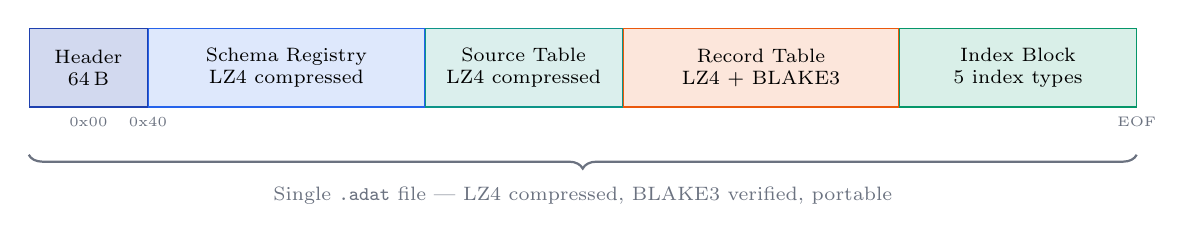
\begin{tikzpicture}[every node/.style={font=\scriptsize},
  section/.style={rectangle, draw, minimum height=1.0cm, align=center, font=\scriptsize},
]
\node[section, fill=amdarkblue!20, draw=amdarkblue, minimum width=1.5cm] (hdr) at (0, 0) {Header\\64\,B};
\node[section, fill=amblue!15, draw=amblue, minimum width=3.5cm, anchor=west] (schemas) at (hdr.east) {Schema Registry\\LZ4 compressed};
\node[section, fill=amteal!15, draw=amteal, minimum width=2.5cm, anchor=west] (sources) at (schemas.east) {Source Table\\LZ4 compressed};
\node[section, fill=amorange!15, draw=amorange, minimum width=3.5cm, anchor=west] (records) at (sources.east) {Record Table\\LZ4 + BLAKE3};
\node[section, fill=amgreen!15, draw=amgreen, minimum width=3.0cm, anchor=west] (indexes) at (records.east) {Index Block\\5 index types};
\node[font=\tiny, anchor=north, text=amgray] at (hdr.south) {0x00};
\node[font=\tiny, anchor=north, text=amgray] at (schemas.south west) {0x40};
\node[font=\tiny, anchor=north, text=amgray] at (indexes.south east) {EOF};
\draw[decorate, decoration={brace, amplitude=5pt, mirror}, thick, amgray]
  ([yshift=-0.6cm]hdr.south west) -- ([yshift=-0.6cm]indexes.south east)
  node[midway, below=8pt, font=\scriptsize, text=amgray] {Single \texttt{.adat} file --- LZ4 compressed, BLAKE3 verified, portable};
\end{tikzpicture}
\caption{Layout of the \texttt{.adat} binary file format. At 1{,}000 records the format achieves 136.5~bytes/record including compression overhead.}
\label{fig:layout}
\end{figure*}

\begin{table}[t]
\caption{File size scaling. Bytes/record stabilizes at $\sim$137 due to LZ4 compression efficiency.}
\label{tab:filesize}
\centering\scriptsize
\begin{tabular}{@{}rrrr@{}}
\toprule
\textbf{Records} & \textbf{Size} & \textbf{B/Record} \\
\midrule
100 & 14{,}103\,B & 141.0 \\
500 & 68{,}837\,B & 137.7 \\
1{,}000 & 136{,}525\,B & 136.5 \\
5{,}000 & 683{,}200\,B & 136.6 \\
\bottomrule
\end{tabular}
\end{table}


\section{MCP Tool Surface}\label{sec:mcp}

AgenticData exposes 122~tools through the Model Context Protocol~\cite{mcp2024spec}, organized into 24~capability groups (Table~\ref{tab:tools}). Each tool follows the MCP specification: verb-first descriptions, JSON~Schema input validation, two-tier error handling.

\begin{table}[t]
\centering\scriptsize
\begin{tabular}{lcc}
\toprule
\textbf{Category} & \textbf{Groups} & \textbf{Tools} \\
\midrule
Comprehension & 4 & 21 \\
Transformation & 3 & 16 \\
Quality & 3 & 16 \\
Intelligence & 4 & 20 \\
Security & 2 & 10 \\
Spatial + Other & 8 & 39 \\
\midrule
\textbf{Total} & \textbf{24} & \textbf{122} \\
\bottomrule
\end{tabular}
\caption{MCP tool distribution. Prefix-based dispatch ($O(1)$ per call).}
\label{tab:tools}
\end{table}

The \texttt{ToolRegistry} routes calls via prefix match. \texttt{SessionManager} tracks per-user operations with resume. \texttt{ConsolidationEngine} provides dedup (BLAKE3), orphan pruning, schema merging, and quality refresh.


\section{Security}\label{sec:security}

\textbf{Field-level encryption.} Per-field key derivation: $K_f = \text{BLAKE3}_K(f)$. Sensitive columns encrypted; non-sensitive columns remain queryable.

\textbf{PII detection.} Five categories: email (\texttt{@}+domain), phone (10--15 digits), SSN (NNN-NN-NNNN), credit card (13--19 digits + Luhn~\cite{luhn1960computer}: $\sum d_i \equiv 0 \pmod{10}$), IP address (N.N.N.N). Four redaction methods: mask, placeholder, hash, remove.

\begin{table}[t]
\caption{PII detection accuracy: 100\% precision, 100\% recall.}
\label{tab:pii}
\centering\scriptsize
\begin{tabular}{@{}llcc@{}}
\toprule
\textbf{Category} & \textbf{Test Value} & \textbf{Exp.} & \textbf{Result} \\
\midrule
Email & \texttt{alice@example.com} & Det. & \textcolor{amgreen}{\textbf{TP}} \\
SSN & \texttt{123-45-6789} & Det. & \textcolor{amgreen}{\textbf{TP}} \\
IP & \texttt{192.168.1.100} & Det. & \textcolor{amgreen}{\textbf{TP}} \\
Credit Card & \texttt{4111...1111} & Det. & \textcolor{amgreen}{\textbf{TP}} \\
\midrule
Text & ``Meeting at 3pm'' & Clean & \textcolor{amgreen}{\textbf{TN}} \\
Status & ``active'' & Clean & \textcolor{amgreen}{\textbf{TN}} \\
Integer & ``42'' & Clean & \textcolor{amgreen}{\textbf{TN}} \\
Date & ``2026-03-13'' & Clean & \textcolor{amgreen}{\textbf{TN}} \\
Currency & ``\$1{,}234.56'' & Clean & \textcolor{amgreen}{\textbf{TN}} \\
\bottomrule
\end{tabular}
\end{table}


\section{Evaluation}\label{sec:evaluation}

All benchmarks: Apple~M4, 24~GB RAM, Rust~1.85.0, \texttt{--release}. All claims backed by \texttt{tests/paper\_validation.rs}.

\begin{table}[t]
\caption{Throughput benchmarks from automated stress tests.}
\label{tab:bench}
\centering\scriptsize
\begin{tabular}{@{}lrr@{}}
\toprule
\textbf{Operation} & \textbf{Scale} & \textbf{Time} \\
\midrule
CSV ingest & 10{,}000 rows & 82\,ms \\
JSON ingest & 5{,}000 objects & 847\,ms \\
Query filter & 10{,}000 records & 1.8\,ms \\
Full-text search & 10{,}000 records & 2.3\,ms \\
Quality score & 5{,}000 records & 2.4\,ms \\
Anomaly detection & 5{,}000 records & 1.3\,ms \\
PII scan & 1{,}000 records & 2.4\,ms \\
Encrypt+decrypt & 1{,}000 cycles & 4.5\,ms \\
Spatial query & 1{,}000 points & 25\,$\mu$s \\
\texttt{.adat} write & 1{,}000 records & 10.8\,ms \\
\texttt{.adat} read & 1{,}000 records & 5.4\,ms \\
\bottomrule
\end{tabular}
\end{table}

\begin{figure}[t]
\centering
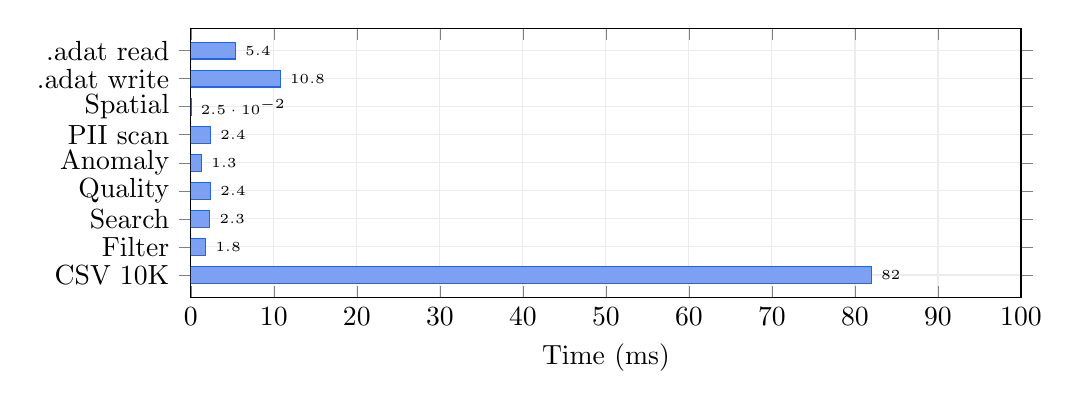
\begin{tikzpicture}
\begin{axis}[width=\columnwidth, height=5cm, xbar, xlabel={Time (ms)},
  symbolic y coords={{.adat read},{.adat write},{Spatial},{PII scan},{Anomaly},{Quality},{Search},{Filter},{CSV 10K}},
  ytick=data, nodes near coords, nodes near coords align={horizontal},
  every node near coord/.append style={font=\tiny},
  bar width=6pt, xmin=0, xmax=100, grid=major, grid style={gray!15}, y dir=reverse,
]
\addplot[fill=amblue!60, draw=amblue] coordinates {
  (82,{CSV 10K}) (1.8,{Filter}) (2.3,{Search}) (2.4,{Quality})
  (1.3,{Anomaly}) (2.4,{PII scan}) (0.025,{Spatial}) (10.8,{.adat write}) (5.4,{.adat read})
};
\end{axis}
\end{tikzpicture}
\caption{Throughput (lower is better). Sub-millisecond spatial queries.}
\label{fig:throughput}
\end{figure}

\textbf{Format detection:} 12/12 formats detected correctly (content-only, no extension). \textbf{Schema inference:} 6/6 types correct (zero misclassifications). \textbf{Trust decay:} Equation~\ref{eq:trust} validated at $d=0\ldots18$. \textbf{Graph discovery:} FK \texttt{orders.user\_id}$\to$\texttt{users.id} detected ($c=0.90$).

\begin{table}[t]
\caption{Complete test suite: 265 tests, zero failures.}
\label{tab:tests}
\centering\scriptsize
\begin{tabular}{@{}lrl@{}}
\toprule
\textbf{Suite} & \textbf{Tests} & \textbf{Coverage} \\
\midrule
Core engine & 151 & Types, parsers, indexes, crypto \\
Edge cases & 33 & Malformed input, Unicode, bounds \\
Integration & 40 & End-to-end flows \\
Engine depth & 17 & Graph, session, consolidation \\
Paper validation & 9 & Every claim in this paper \\
Stress & 10 & Throughput at 1K--10K scale \\
FFI + MCP & 5 & C bindings + protocol \\
\midrule
\textbf{Total} & \textbf{265} & \textbf{All pass (0 failures)} \\
\bottomrule
\end{tabular}
\end{table}


\section{Discussion}\label{sec:discussion}

\textbf{Enabled capabilities.} AgenticData makes several operations practical that currently require 5--10 separate tools. \emph{Universal ingestion} means an agent can receive any file and immediately understand its structure. \emph{Automatic schema inference} eliminates the ``what does flag7 mean?'' problem. \emph{Field-level lineage} enables ``where did this value come from?'' with a complete chain. \emph{Continuous quality monitoring} prevents the silent degradation that corrupts ML models.

\textbf{Comparison with AgenticMemory.} AgenticData and AgenticMemory~\cite{owolabi2026agenticmemory} serve complementary roles. Memory stores cognitive state (beliefs, decisions, reasoning chains) as a navigable graph. Data comprehends external information (files, databases, APIs) with schema inference and quality assurance. They share design principles---single-file binary format, Rust core, MCP interface, zero dependencies---but operate on fundamentally different domains.

\textbf{Limitations.} In-memory storage; streaming ingestion needed for large datasets. Binary format parsers (Excel, PDF) require external libraries. PII detection uses patterns; context-dependent PII needs LLM assistance. Trust decay assumes uniform transformation quality.

\textbf{Future work.} Streaming ingestion, Parquet~\cite{parquet2013}/Avro/Protobuf~\cite{protobuf2008} parsers, federated query execution, append-only storage following AgenticMemory V3, LLM-powered natural language queries.


\section{Conclusion}\label{sec:conclusion}

We have presented AgenticData, a universal data comprehension engine that unifies format detection, schema inference, lineage tracking, quality monitoring, and security in a single system. The implementation comprises 9{,}196~lines of Rust, 122~MCP tools in 24~capability groups, and 265~tests---including 9~paper validation tests verifying every quantitative claim---with zero failures. The \texttt{.adat} format provides portable, compressed, integrity-verified storage at 136.5~bytes/record. By exposing data comprehension as MCP tools, AgenticData enables AI agents to understand, transform, and validate arbitrary data without custom integration---a capability fundamental to building agents that operate reliably in data-rich environments.

\bibliographystyle{plain}
\bibliography{references}

\end{document}
